\section*{4. Metodología}

Para el desarrollo de este proyecto se evaluaron diferentes metodologías ágiles, siendo las principales candidatas Scrum y Kanban. A continuación se presenta el análisis comparativo que justifica la elección final.

\subsection{4.1 Evaluación de Scrum}

\subsubsection{Ventajas consideradas:}

\begin{itemize}
    \item Metodología ágil más utilizada en la industria del desarrollo software.
    \item Sprints de tiempo fijo con entregas incrementales, muy útil para forzar la constancia y el trabajo continuo.
    \item Ceremonias estructuradas (Sprint Planning, Daily Scrum, Sprint Review, Retrospective) que permiten la correcta gestión del proyecto.
    \item Estimaciones de tiempo que facilitan la planificación.
\end{itemize}

\subsubsection{Inconvenientes para este proyecto:}

\begin{itemize}
    \item Scrum está diseñado para equipos, no para desarrollo individual. Los roles (Product Owner, Scrum Master, Developer) resultan artificiales cuando el desarrollador es una única persona.
    \item Las ceremonias diarias (por ejemplo, el Daily Scrum) carecen de sentido práctico en contexto individual.
    \item Rigidez de los sprints: Una vez iniciado el sprint, no se pueden modificar los objetivos ni las tareas seleccionadas hasta su finalización.
\end{itemize}

\subsubsection{Motivos de descarte:}

La naturaleza individual del proyecto y la ausencia de entregas incrementales intermedias hacen que Scrum introduzca complejidad innecesaria sin aportar beneficios reales. Adaptar artificialmente los roles y ceremonias no representa fielmente cómo se desarrolló el proyecto.

\subsection{4.2 Metodología seleccionada: Kanban}

Kanban es una metodología ágil basada en flujo continuo de trabajo que visualiza el proceso mediante un tablero dividido en columnas que representan estados de las tareas. No utiliza iteraciones de tiempo fijo ni roles predefinidos.

\subsubsection{Estructura del tablero Kanban implementado:}

\begin{itemize}
    \item \textbf{Backlog:} tareas pendientes de iniciar
    \item \textbf{To Do:} tareas priorizadas para desarrollo inmediato
    \item \textbf{In Progress:} tareas en desarrollo activo (límite Work In Progress: 3 tareas)
    \item \textbf{Done:} tareas completadas y validadas
\end{itemize}

\subsubsection{Ventajas para este proyecto:}

\begin{itemize}
    \item \textbf{Flexibilidad adaptativa:} Permite reordenar prioridades según descubrimientos técnicos o cambios en requisitos sin violar reglas metodológicas.
    \item \textbf{Flujo natural:} Se adapta al ritmo real de trabajo individual sin imposiciones de tiempo o plazos de entrega intermedios.
    \item \textbf{Visualización clara:} El tablero proporciona instantáneamente el estado del proyecto.
\end{itemize}

\subsubsection{Desventajas asumidas:}

\begin{itemize}
    \item Menor estructura formal para métricas de velocidad.
    \item Requiere disciplina personal para mantener límites WIP y actualizar el tablero.
\end{itemize}

Kanban resulta más apropiado para el contexto de este TFG al tratarse de un proyecto de desarrollo individual 
sin entregas intermedias formales. La flexibilidad de Kanban permite adaptarse a las
 necesidades reales del proyecto manteniendo trazabilidad completa del proceso. Además, 
 al no estar sujeto a sprints de tiempo fijo, se facilita la gestión temporal del
  proyecto en coordinación con otras asignaturas del grado, permitiendo ajustar la carga de
   trabajo según períodos de exámenes, entregas de otras materias y disponibilidad personal, 
   algo que la rigidez de los sprints de Scrum dificultaría considerablemente.

\subsubsection{Implementación de Kanban}

\textbf{Herramienta utilizada:} GitHub Projects
\textbf{Herramienta de monitorización:} Clockify

\textbf{Límites WIP aplicados:}
\begin{itemize}
    \item Máximo 3 tareas en ``In Progress'' simultáneamente
\end{itemize}

\textbf{Priorización:} Las tareas del Backlog se priorizaron y planifican según dependencias técnicas y criticidad funcional.

\subsection{4.3 Planificación Temporal}

\textbf{Herramienta de planificación:} Microsoft Project
\textbf{Herramienta de monitorización:} Clockify

\textbf{Parámetros de planificación:}
\begin{itemize}
    \item Rol único: Developer
    \item Jornada laboral: 4 horas diarias
    \item Duración total estimada: 19 semanas
\end{itemize}

El diagrama de Gantt generado (ver Figura 5) muestra la distribución temporal de las diferentes fases del proyecto: análisis y diseño inicial, desarrollo de módulos principales, integración, pruebas y documentación final.

A pesar de que el estándar habitual de una jornada de trabajo se establece en 8 horas diarias, en la planificación de este proyecto se ha considerado cada día como equivalente a 4 horas de trabajo efectivo. Esta decisión se debe a que no resulta realista asumir una dedicación diaria de 8 horas completas al TFG, dado que este se desarrolla en paralelo con otras asignaturas del grado que también requieren una inversión significativa de tiempo y esfuerzo.

\begin{figure}[H]
\centering
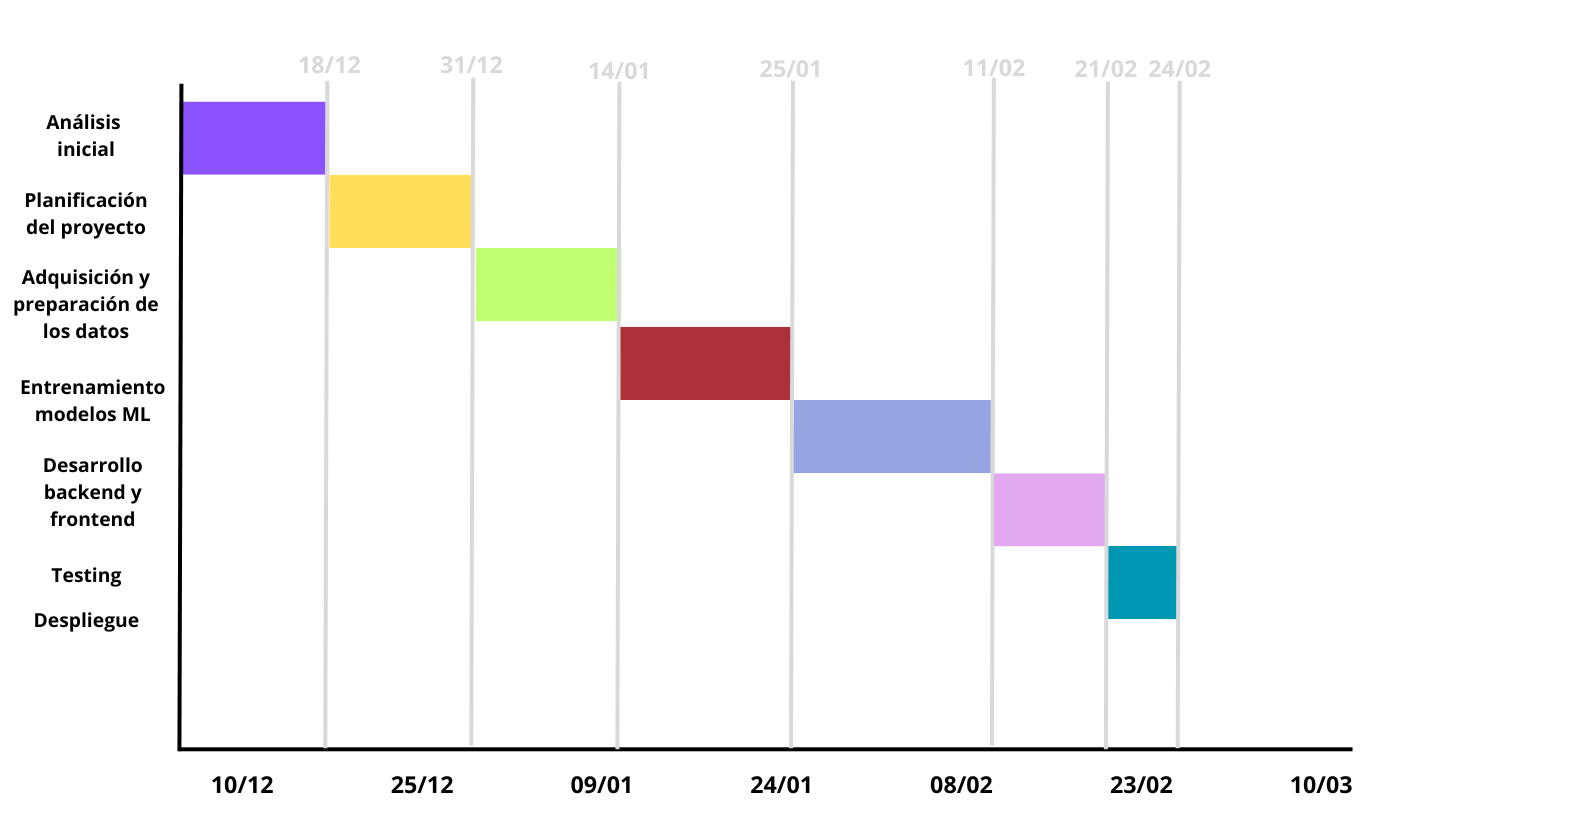
\includegraphics[width=0.9\textwidth]{images/gantt.png}
\label{fig:gantt}
\caption{Diagrama de Gantt de la línea base del cronograma.}
\end{figure}

\subsection{4.4 EDT (Estructura Desglose de Trabajo)}

A continuación, se presenta la Estructura de Desglose de Trabajo (EDT), que organiza el trabajo en paquetes manejables y define la base lógica sobre la que se asientan las actividades y recursos detallados en el diccionario de la EDT posterior.
\begin{figure}[H]
\centering
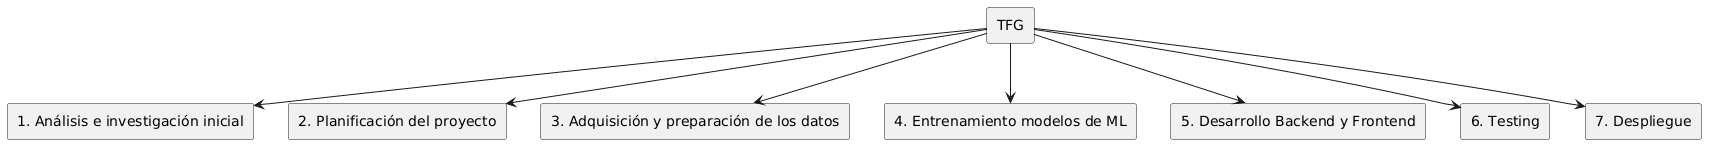
\includegraphics[width=0.9\textwidth]{images/edt.png}
\caption{Estructura de Desglose de Trabajo (EDT) del proyecto.}
\label{fig:edt}
\end{figure}

\subsubsection{Diccionario de la EDT}

\textbf{Id: 1}

\textbf{Nombre paquete:} Análisis e investigación inicial

\textbf{Descripción:} Investigación y análisis de proyectos existentes relacionados con predicción deportiva y aplicación de machine learning en fútbol, con el objetivo de identificar buenas prácticas, limitaciones y oportunidades de mejora.

\textbf{Actividades}

\begin{center}
\small
\begin{tabular}{|p{0.45\textwidth}|p{0.25\textwidth}|p{0.25\textwidth}|}
\hline
\textbf{Actividad} & \textbf{Duración} & \textbf{Recurso} \\
\hline
A1 - Estudio proyectos similares & 4 días & Google Chrome, Github \\
\hline
A2 - Investigación fuentes de datos & 2 días & Google Chrome \\
\hline
A3 - Evaluar viabilidad web scraping & 2 días & Google Chrome, documentación técnica \\
\hline
A4 - Análisis de competidores & 4 días & Google Chrome \\
\hline
\end{tabular}
\end{center}

\vspace{0.5cm}

\textbf{Id: 2}

\textbf{Nombre paquete:} Planificación del proyecto

\textbf{Descripción:} Definición formal del alcance del proyecto, especificación de requisitos funcionales y no funcionales, historias de usuario y planificación detallada de recursos y cronograma.

\textbf{Actividades}

\begin{center}
\small
\begin{tabular}{|p{0.45\textwidth}|p{0.25\textwidth}|p{0.25\textwidth}|}
\hline
\textbf{Actividad} & \textbf{Duración} & \textbf{Recurso} \\
\hline
A5 - Definición del alcance del proyecto & 2 días & Google Docs \\
\hline
A6 - Especificación Requisitos Funcionales y no Funcionales & 2 días & Google Docs \\
\hline
A7 - Definición historias de usuario y mockups & 3 días & Google Docs \\
\hline
A8 - Elección stack tecnológico & 2 días & Documentación técnica \\
\hline
A9 - Planificación temporal y de recursos & 2 días & MS Project \\
\hline
\end{tabular}
\end{center}

\vspace{0.5cm}

\textbf{Id: 3}

\textbf{Nombre paquete:} Adquisición y preparación de los datos

\textbf{Descripción:} Obtención de datos mediante web scraping de las fuentes identificadas, almacenamiento en formato CSV y preprocesamiento para su posterior uso en modelos de machine learning. Esta fase incluye limpieza de datos, tratamiento de valores nulos, normalización.

\textbf{Actividades}

\begin{center}
\small
\begin{tabular}{|p{0.45\textwidth}|p{0.25\textwidth}|p{0.25\textwidth}|}
\hline
\textbf{Actividad} & \textbf{Duración} & \textbf{Recurso} \\
\hline
A10 - Desarrollo scripts de scrapping & 6 días & VS Code, Python, pandas \\
\hline
A11 - Matching de datos & 2 días & VS Code, Python, pandas \\
\hline
A12 - Almacenamiento en formato CSV & 1 día & VS Code, Python, pandas \\
\hline
A13 - Preprocesamiento y limpieza de datos & 6 días & VS Code, Python, pandas, numpy \\
\hline
\end{tabular}
\end{center}

\vspace{0.5cm}

\textbf{Id: 4}

\textbf{Nombre paquete:} Entrenamiento modelos de ML

\textbf{Descripción:} Selección, entrenamiento y optimización de modelos predictivos para la evaluación del rendimiento de jugadores. Se implementan técnicas de validación cruzada, ajuste de hiperparámetros mediante Grid Search y técnicas de explicabilidad XAI para garantizar predicciones precisas y comprensibles.

\textbf{Actividades}

\begin{center}
\small
\begin{tabular}{|p{0.45\textwidth}|p{0.25\textwidth}|p{0.25\textwidth}|}
\hline
\textbf{Actividad} & \textbf{Duración} & \textbf{Recurso} \\
\hline
A14 - Selección algoritmos candidatos & 1 día & VS Code, documentación de scikit-learn \\
\hline
A15 - Entrenamiento inicial de los modelos & 2 días & VS Code, Python, scikit-learn \\
\hline
A16 - Ajuste de hiperparámetros, validación cruzada y evaluación & 12 días & VS Code, Python, scikit-learn \\
\hline
A17 - Investigación e implementación XAI & 6 días & VS Code, Python, Chrome \\
\hline
\end{tabular}
\end{center}

\vspace{0.5cm}

\textbf{Id: 5}

\textbf{Nombre paquete:} Desarrollo Backend y Frontend

\textbf{Descripción:} Selección, entrenamiento y optimización de modelos predictivos para la evaluación del rendimiento de jugadores. Se implementan técnicas de validación cruzada, ajuste de hiperparámetros mediante Grid Search y técnicas de explicabilidad XAI para garantizar predicciones precisas y comprensibles.

\textbf{Actividades}

\begin{center}
\small
\begin{tabular}{|p{0.45\textwidth}|p{0.25\textwidth}|p{0.25\textwidth}|}
\hline
\textbf{Actividad} & \textbf{Duración} & \textbf{Recurso} \\
\hline
A18 - Configuración inicial del proyecto & 1 día & VS Code, Django \\
\hline
A19 - Diseño de la arquitectura final & 2 días & Mermaid \\
\hline
A20 - Modelado de la BD & 4 días & Mermaid \\
\hline
A21 - Desarrollo vistas y templates & 10 días & VS Code, Python, Django \\
\hline
\end{tabular}
\end{center}

\vspace{0.5cm}

\textbf{Id: 6}

\textbf{Nombre paquete:} Testing

\textbf{Descripción:} Verificación del correcto funcionamiento del sistema mediante pruebas unitarias, pruebas sobre la lógica de obtención y combinación de datos, y pruebas sobre las vistas de la aplicación web, con el objetivo de garantizar la calidad del software antes del despliegue.

\textbf{Actividades}

\begin{center}
\small
\begin{tabular}{|p{0.45\textwidth}|p{0.25\textwidth}|p{0.25\textwidth}|}
\hline
\textbf{Actividad} & \textbf{Duración} & \textbf{Recurso} \\
\hline
A22 - Pruebas unitarias de funcionalidades clave & 6 días & VS Code, pytest \\
\hline
A23 - Pruebas de consistencia de los datos & 2 días & VS Code, Python \\
\hline
A24 - Corrección de errores & 4 días & VS Code, Python \\
\hline
\end{tabular}
\end{center}

\vspace{0.5cm}

\textbf{Id: 7}

\textbf{Nombre paquete:} Despliegue

\textbf{Descripción:} Configuración del entorno de producción y despliegue de la aplicación en una plataforma cloud accesible a través de contenedores de Docker.

\textbf{Actividades}

\begin{center}
\small
\begin{tabular}{|p{0.45\textwidth}|p{0.25\textwidth}|p{0.25\textwidth}|}
\hline
\textbf{Actividad} & \textbf{Duración} & \textbf{Recurso} \\
\hline
A25 - Configuración del entorno de producción & 2 días & Docker, DockerHub \\
\hline
A26 - Despliegue & 1 día & Microsoft Azure \\
\hline
\end{tabular}
\end{center}

\subsection{4.5 Planificación de riesgos}

Para asegurar el éxito del proyecto, se ha llevado a cabo una identificación y evaluación de los posibles riesgos que podrían impactar en el desarrollo, estimando su probabilidad de ocurrencia y su impacto en el cronograma o alcance.

\subsubsection{Identificación y Matriz de Riesgos}

\begin{figure}[H]
\centering
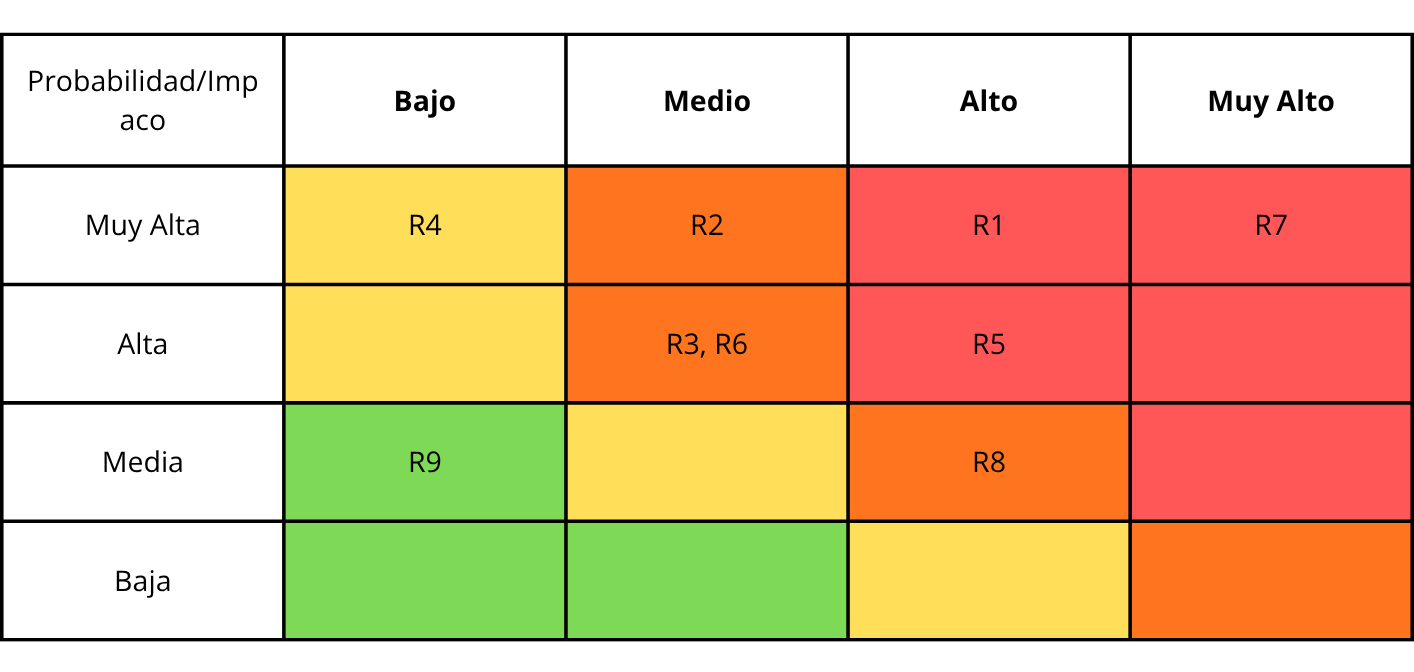
\includegraphics[width=0.9\textwidth]{images/riesgos.png}
\caption{Matriz de riesgos del proyecto.}
\label{fig:riesgos}
\end{figure}

\vspace{0.5cm}

\begin{center}
\small
\setlength{\tabcolsep}{6pt}
\begin{tabular}{|p{0.08\textwidth}|p{0.35\textwidth}|p{0.25\textwidth}|p{0.22\textwidth}|}
\hline
\textbf{ID} & \textbf{Nombre} & \textbf{Probabilidad} & \textbf{Impacto} \\
\hline
R1 & Restricciones en la obtención de datos & Muy alta & Alta \\
\hline
\multicolumn{4}{|p{0.9\textwidth}|}{\textbf{Descripción:} Imposibilidad de extraer ciertos datos debido a bloqueos de IP, captchas, APIs limitadas o cambios estructurales en el DOM de las páginas fuente.} \\
\hline
\multicolumn{4}{|p{0.9\textwidth}|}{\textbf{Plan de mitigación:} Se implementarán buenas prácticas de scraping (tiempos de espera aleatorios, cabeceras User-Agents). Como contingencia, si el bloqueo es total, se buscarán alternativas web o descargarán y almacenarán los HTML manualmente.} \\
\hline
\end{tabular}
\end{center}

\vspace{0.3cm}

\begin{center}
\small
\setlength{\tabcolsep}{6pt}
\begin{tabular}{|p{0.08\textwidth}|p{0.35\textwidth}|p{0.25\textwidth}|p{0.22\textwidth}|}
\hline
\textbf{ID} & \textbf{Nombre} & \textbf{Probabilidad} & \textbf{Impacto} \\
\hline
R2 & Rendimiento predictivo deficiente & Media & Muy Alto \\
\hline
\multicolumn{4}{|p{0.9\textwidth}|}{\textbf{Descripción:} Existe la incertidumbre de que los modelos de Machine Learning no logren una precisión o capacidad predictiva aceptable con los datos proporcionados.} \\
\hline
\multicolumn{4}{|p{0.9\textwidth}|}{\textbf{Plan de mitigación y contingencia:} Si las métricas iniciales son deficientes, se realizará una iteración extra de Feature Engineering (creación de nuevas variables derivadas). Si el límite predictivo de los datos se mantiene bajo, la contingencia es cambiar el enfoque del TFG hacia el análisis y la investigación: en lugar de prometer una herramienta infalible, el valor del proyecto residirá en la comparativa exhaustiva de los algoritmos y en documentar científicamente por qué ciertas variables no son determinantes para predecir el rendimiento deportivo.} \\
\hline
\end{tabular}
\end{center}

\vspace{0.3cm}

\begin{center}
\small
\begin{tabular}{|p{0.08\textwidth}|p{0.35\textwidth}|p{0.25\textwidth}|p{0.22\textwidth}|}
\hline
\textbf{ID} & \textbf{Nombre} & \textbf{Probabilidad} & \textbf{Impacto} \\
\hline
R3 & Solapamiento de calendario académico & Alta & Medio \\
\hline
\multicolumn{4}{|p{0.9\textwidth}|}{\textbf{Descripción:} Picos de trabajo por entregas o exámenes de otras asignaturas que reduzcan la disponibilidad de 4 horas diarias previstas.} \\
\hline
\multicolumn{4}{|p{0.9\textwidth}|}{\textbf{Plan de mitigación:} La elección metodológica de Kanban absorbe este riesgo al carecer de sprints rígidos. Permite pausar y reanudar tareas según la carga lectiva sin romper la planificación metodológica.} \\
\hline
\end{tabular}
\end{center}

\vspace{0.3cm}

\begin{center}
\small
\begin{tabular}{|p{0.08\textwidth}|p{0.35\textwidth}|p{0.25\textwidth}|p{0.22\textwidth}|}
\hline
\textbf{ID} & \textbf{Nombre} & \textbf{Probabilidad} & \textbf{Impacto} \\
\hline
R4 & Manejo de dependencias cruzadas & Muy Alta & Bajo \\
\hline
\multicolumn{4}{|p{0.9\textwidth}|}{\textbf{Descripción:} Conflictos de compatibilidad entre las diferentes versiones de librerías de Machine Learning (scikit-learn, pandas, numpy) y el entorno del framework web (Django).} \\
\hline
\multicolumn{4}{|p{0.9\textwidth}|}{\textbf{Plan de mitigación:} Mitigación mediante el uso estricto de entornos virtuales desde el primer día, aislando el entorno de datos del entorno web hasta su integración, y congelando las versiones estables en un archivo requirements.txt.} \\
\hline
\end{tabular}
\end{center}

\vspace{0.3cm}

\begin{center}
\small
\begin{tabular}{|p{0.08\textwidth}|p{0.35\textwidth}|p{0.25\textwidth}|p{0.22\textwidth}|}
\hline
\textbf{ID} & \textbf{Nombre} & \textbf{Probabilidad} & \textbf{Impacto} \\
\hline
R5 & Integración de modelos ML en el backend & Alta & Alto \\
\hline
\multicolumn{4}{|p{0.9\textwidth}|}{\textbf{Descripción:} Desconocimiento inicial sobre la arquitectura óptima para guardar los modelos entrenados, cargarlos y realizar inferencias desde Django de manera eficiente.} \\
\hline
\multicolumn{4}{|p{0.9\textwidth}|}{\textbf{Plan de mitigación:} Realizar una fase inicial de investigación sobre las prácticas recomendadas para almacenar y cargar modelos de aprendizaje automático en aplicaciones web con Django. Para ello, se revisará la documentación oficial de frameworks utilizados y ejemplos de integración con Django.} \\
\hline
\end{tabular}
\end{center}

\vspace{0.3cm}

\begin{center}
\small
\begin{tabular}{|p{0.08\textwidth}|p{0.35\textwidth}|p{0.25\textwidth}|p{0.22\textwidth}|}
\hline
\textbf{ID} & \textbf{Nombre} & \textbf{Probabilidad} & \textbf{Impacto} \\
\hline
R6 & Curva de aprendizaje de XAI & Alta & Medio \\
\hline
\multicolumn{4}{|p{0.9\textwidth}|}{\textbf{Descripción:} La implementación de técnicas de XAI puede presentar una curva de aprendizaje más pronunciada de lo estimado inicialmente.} \\
\hline
\multicolumn{4}{|p{0.9\textwidth}|}{\textbf{Plan de mitigación:} Se comenzará integrando las herramientas de XAI más documentadas en la industria (como SHAP). Si el tiempo apremia, se reducirá el alcance de la explicabilidad.} \\
\hline
\end{tabular}
\end{center}

\vspace{0.3cm}

\begin{center}
\small
\begin{tabular}{|p{0.08\textwidth}|p{0.35\textwidth}|p{0.25\textwidth}|p{0.22\textwidth}|}
\hline
\textbf{ID} & \textbf{Nombre} & \textbf{Probabilidad} & \textbf{Impacto} \\
\hline
R7 & Coste temporal en el matching y procesamiento de datos & Muy Alta & Muy alto \\
\hline
\multicolumn{4}{|p{0.9\textwidth}|}{\textbf{Descripción:} Dificultad para cruzar datos de diferentes fuentes (por ejemplo, discrepancias en la nomenclatura de los nombres de los jugadores o equipos), lo que puede consumir gran parte de la fase de preparación.} \\
\hline
\multicolumn{4}{|p{0.9\textwidth}|}{\textbf{Plan de mitigación:} En lugar de hacer cruces manuales o exactos, se programarán mecanismos utilizando librerías específicas como FuzzyWuzzy o TheFuzz, complementados con diccionarios manuales únicamente para los casos extremos.} \\
\hline
\end{tabular}
\end{center}

\vspace{0.3cm}

\begin{center}
\small
\begin{tabular}{|p{0.08\textwidth}|p{0.35\textwidth}|p{0.25\textwidth}|p{0.22\textwidth}|}
\hline
\textbf{ID} & \textbf{Nombre} & \textbf{Probabilidad} & \textbf{Impacto} \\
\hline
R8 & Rendimiento deficiente en producción & Media & Alto \\
\hline
\multicolumn{4}{|p{0.9\textwidth}|}{\textbf{Descripción:} Tiempos de respuesta lentos o caídas por falta de memoria al intentar cargar y ejecutar los modelos de ML una vez la aplicación esté desplegada en un servidor en la nube.} \\
\hline
\multicolumn{4}{|p{0.9\textwidth}|}{\textbf{Plan de mitigación:} Para evitar que la web sea lenta, la arquitectura se diseñará para cargar el modelo de Machine Learning en la memoria del servidor una sola vez durante el arranque de la aplicación (ej. instanciándolo en el archivo apps.py de Django) y no en cada petición HTTP del usuario. Si los recursos del servidor gratuito son insuficientes, se optará por desplegar versiones más ligeras de los modelos (menos profundidad de árboles o menos parámetros, sacrificando algo de precisión).} \\
\hline
\end{tabular}
\end{center}

\vspace{0.3cm}

\begin{center}
\small
\begin{tabular}{|p{0.08\textwidth}|p{0.35\textwidth}|p{0.25\textwidth}|p{0.22\textwidth}|}
\hline
\textbf{ID} & \textbf{Nombre} & \textbf{Probabilidad} & \textbf{Impacto} \\
\hline
R9 & Desactualización del dataset & Media & Bajo \\
\hline
\multicolumn{4}{|p{0.9\textwidth}|}{\textbf{Descripción:} Al estar analizando datos de una competición deportiva en curso, cada fin de semana se generan nuevos datos. Existe el riesgo de que, para la fecha de la defensa, el modelo no incluya los últimos partidos o fichajes recientes.} \\
\hline
\multicolumn{4}{|p{0.9\textwidth}|}{\textbf{Plan de mitigación:} Definir en el alcance del proyecto una ``fecha de corte'' clara (por ejemplo, ``datos extraídos hasta la jornada 17''). Se trabajará con un dataset cerrado.} \\
\hline
\end{tabular}
\end{center}

\subsection{4.6 Gestión de la Calidad}

Para garantizar que el software desarrollado sea mantenible, escalable y libre de errores críticos, se han establecido las siguientes métricas y herramientas de calidad:

\begin{itemize}
    \item \textbf{Análisis estático de código:} Se integrará SonarQube para evaluar continuamente la calidad del código. Esta herramienta detectará vulnerabilidades (security hotspots), code smells y código duplicado, asegurando que se cumplen los estándares de la industria.
\end{itemize}

\subsection{4.7 Análisis de tiempos, costes y desviaciones}

Tal y como se estableció en la planificación temporal, la jornada de trabajo estándar para 
este proyecto se fijó en 4 horas diarias, adaptándose a la realidad de la carga lectiva 
 grado. 
 
 Durante el desarrollo, esta premisa se ha cumplido de forma general, con la excepción
  del periodo vacacional de Navidad (del 24 de diciembre al 30 de enero). La mayor disponibilidad de tiempo en esas fechas permitió acelerar el ritmo de trabajo, logrando completar tareas en una menor cantidad de días calendario, aunque el volumen de horas de trabajo invertidas se mantuvo acorde a las estimaciones.

Para garantizar el éxito del proyecto y mitigar posibles solapamientos con entregas o exámenes de otras asignaturas, la estrategia principal de planificación consistió en concentrar el desarrollo para finalizar a finales de febrero. Esto proporcionó un amplio margen de holgura temporal en caso de no poder cumplir el primer plazo establecido.

\subsubsection{Resumen Temporal y Desviaciones Globales}

A continuación, se presenta la comparativa entre la línea base del proyecto planificada y la ejecución real:

\begin{center}
\small
\begin{tabularx}{\textwidth}{Xccc}
\toprule
\textbf{Parámetro} & \textbf{Planificación Inicial} & \textbf{Ejecución Real} & \textbf{Desviación} \\
\midrule
Fecha de inicio & 10/12/2025 & 10/12/2025 & -- \\
Fecha de fin & 12/03/2026 & 07/04/2026 & + 26 días naturales \\
Horas de trabajo total & 364 h & 384 h & + 20 h \\
Días de trabajo efectivo (4h/día) & 91 días & 96 días & + 5 días efectivos \\
\bottomrule
\end{tabularx}
\end{center}

Como se observa en los datos, el esfuerzo total del proyecto solo sufrió un incremento de 20 horas (equivalentes a 5 jornadas de trabajo de 4 horas). A nivel de calendario, la finalización se desplazó hasta el 7 de abril. Gracias al gran margen de holgura planificado desde el principio, este desplazamiento temporal fue absorbido íntegramente sin poner en riesgo la entrega ni la defensa del proyecto. 
\subsubsection{Comparativa de esfuerzo por paquetes de trabajo}

En la siguiente tabla se desglosa el esfuerzo por cada paquete de la Estructura de Desglose de Trabajo (EDT), evidenciando dónde se produjeron las desviaciones:

\begin{center}
\small
\begin{tabularx}{\textwidth}{cXccc}
\toprule
\textbf{ID} & \textbf{Paquete de Trabajo} & \textbf{Horas Previstas} & \textbf{Horas Reales} & \textbf{Desviación} \\
\midrule
1 & Análisis e investigación inicial & 48 h & 48 h & 0 h \\
2 & Planificación del proyecto & 80 h & 48 h & -32 h \\
3 & Adquisición y preparación de datos & 60 h & 76 h & +16 h \\
4 & Entrenamiento modelos de ML & 48 h & 68 h & +20 h \\
5 & Desarrollo Backend y Frontend & 68 h & 88 h & +20 h \\
6 & Testing & 48 h & 28 h & -20 h \\
7 & Despliegue & 12 h & 28 h & +16 h \\
\midrule
 & TOTAL & 364 h & 384 h & +20 h \\
\bottomrule
\end{tabularx}
\end{center}

Todas las entradas de la herramienta Clockify se pueden consultar en el Apéndice II-Clockify.

\subsubsection{Análisis de desviaciones}

Al comparar la planificación inicial con el tiempo real invertido, se observan variaciones inherentes a la naturaleza de un proyecto que combina ingeniería de software y machine learning. Las diferencias más significativas se concentraron en las siguientes áreas:

\begin{itemize}
    \item \textbf{Fase de entrenamiento y optimización:} las tareas relacionadas con el ajuste de features, hiperparámetros, validación cruzada y evaluación requirieron 48 horas frente a las 32 estimadas. Esto refleja la dificultad de acotar temporalmente las fases de experimentación, donde los resultados obligan a realizar múltiples iteraciones, pruebas y refinamientos hasta alcanzar la precisión deseada en el modelo.
    \item \textbf{Desarrollo de vistas y templates (Frontend/Backend):} Su implementación alcanzó un total de 60 horas (frente a las 40 iniciales) debido al desarrollo iterativo necesario para integrar correctamente la lógica de los modelos predictivos en la interfaz visual.
    \item \textbf{Compensación de tiempos:} Por el contrario, fases como la planificación del proyecto (estimada de forma muy conservadora en 80 h) o el testing requirieron menos dedicación de la prevista inicialmente, lo que ayudó a equilibrar el balance global de horas.
\end{itemize}

\subsubsection{Estimación Económica y Desglose de Costes}

Para calcular el coste del desarrollo, se ha tomado como referencia la tarifa de un perfil profesional de Analista programador J2EE / Web, representativo del estándar de la industria de software. Los datos provienen del "Informe final sobre la consulta preliminar del mercado" de la Junta de Andalucía y disponible en la web de TFG de la ETSII US. En dicho documento, la media acotada para este perfil oscila entre los 28,37 €/hora para perfiles Junior y los 33,43 €/hora para perfiles Senior, por lo que se ha establecido un valor medio de 31 €/hora para este proyecto.

A diferencia de las estimaciones basadas únicamente en salarios brutos, este valor de 31 €/hora representa el precio/hora sin IVA que las empresas del sector facturan habitualmente a la Administración Pública. Al tratarse de una tarifa de licitación para la prestación de servicios profesionales, este importe ya integra de forma intrínseca todos los costes laborales asociados, incluyendo la Seguridad Social a cargo de la empresa, así como los gastos de estructura, herramientas, licencias y el beneficio industrial.

Por este motivo, la cifra empleada constituye una aproximación realista del coste total de mercado. Al cubrir ya todas las cargas sociales y costes indirectos dentro de la propia tarifa horaria de facturación, resulta innecesario aplicar factores correctores o porcentajes adicionales sobre el cálculo final.

Además del coste de personal, se han contemplado los siguientes gastos operativos y de capital:

\textbf{CAPEX (Capital Expenditure):}
\begin{itemize}
   \item \textbf{Amortización de equipo informático:} Según las tablas de la AEAT 2026, los equipos para tratamiento de información tienen un coeficiente de amortización lineal máximo del 26\% anual. Para un ordenador de 1.200 €, la amortización imputada por las 17 semanas de duración del proyecto se calcula como: $1.200 \times 0,26 \times (17/52) = 102,00$ €. Se establece un coste fijo de \textbf{102 €}.
\end{itemize}

\textbf{OPEX (Operational Expenditure):}
\begin{itemize}
    \item Uso de herramientas externas y servicios cloud. Esto incluye el control de versiones mediante GitHub (plan Team, 4 €/usuario/mes), herramientas de Inteligencia Artificial como Gemini Pro (aprox. 20 €/mes), y el despliegue de la aplicación mediante contenedores Docker sobre Microsoft Azure (App Service y Container Registry), con un coste estimado de 30 €/mes.
    \item No obstante, gracias a la disponibilidad de licencias educativas y el programa Azure for Students, el coste real aplicado al proyecto ha sido de 0 €, lo que supone un ahorro aproximado de 216 € durante los cuatro meses de desarrollo.
\end{itemize}

\subsubsection{Cálculo de costes}

Aplicando las premisas anteriores a las horas reales de trabajo:

\begin{center}
\small
\begin{tabularx}{\textwidth}{Xcc}
\toprule
\textbf{Concepto de Gasto} & \textbf{Coste Planificado (364 h)} & \textbf{Coste Real (384 h)} \\
\midrule
Coste Personal (Horas $\times$ 31) € & 11.284,00 € & 11.904,00 € \\
CAPEX (Amortización de equipo) & 102,00 € & 102,00 € \\
OPEX (Licencias e Infraestructura Cloud) & 0,00 €* & 0,00 €* \\
\midrule
COSTE TOTAL DEL PROYECTO & 11.386,00 € & 12.006,00 € \\
\bottomrule
\end{tabularx}
\end{center}

\noindent (Nota: Sin la aplicación de licencias educativas, el OPEX ascendería a 216 € en total).

El coste final de desarrollo del Trabajo de Fin de Grado asciende a 12.006,00 €, lo que supone un incremento de 620,00 € respecto a lo estimado inicialmente, derivado principalmente del aumento de horas en las fases de entrenamiento de modelos y desarrollo.

\subsubsection{Reserva de Contingencia}

Atendiendo a las buenas prácticas en la dirección y gestión de proyectos, no es recomendable establecer un presupuesto cerrado sin margen de maniobra. Por ello, se ha establecido una reserva de contingencia del 10 \% sobre el coste total final:

\textbf{Reserva de contingencia:} 1.200,60 €

Por tanto, el presupuesto final estimado con el que se debería dotar al proyecto para garantizar su viabilidad técnica y económica asciende a:

\begin{center}
\Large 13.206,60 €
\end{center}

